\documentclass[12pt]{article}
\usepackage[a4paper,
            inner=10mm,
            outer=50mm, % = marginparsep + marginparwidth 
                       %   + 5mm (between marginpar and page border)
            top=20mm,
            bottom=25mm,
            marginparsep=5mm,
            marginparwidth=40mm,
            % showframe
            ]{geometry}
\usepackage{amsfonts}
\usepackage{amsmath}
\usepackage{xcolor}
\usepackage{todonotes}
\usepackage{pythonhighlight}

% define command for grey colored text
% \newcommand{\note}[1]{ \textit{\textcolor{gray}{... #1 ...}} }
\newcommand{\note}[1]{\todo[color=yellow!40,bordercolor=none,linecolor=black]{#1}}
\tolerance=1
\emergencystretch=\maxdimen
\hyphenpenalty=10000
\hbadness=10000

\begin{document}

\listoftodos

\section{Introduction}

\note{8 - 10 pages of introduction}

\textbf{Deep Learning (DL)} is a branch of \textbf{Artificial Intelligence (AI)} that emphasizes the use of neural networks to fit the inputs and outputs of a dataset.
The training of a neural network is done by computing the gradients of the loss function with respect to the weights and biases of the network.
A better trained neural network can better approximate the function that maps the inputs to the outputs of the dataset.

\textbf{Reinforcement Learning (RL)} is a branch of AI that emphasizes on solving problems through trials and errors with delayed rewards.
RL had most success in the domain of \textbf{Game Playing}: making agents that could play boardgames, Atari games, or other types of games.
An extension to Game Playing is \textbf{General Game Playing (GGP)}, with the goal of designing agents that could play any type of game without having much prior knowledge of the games.

\textbf{Deep Reinforcement Learning (DRL)} is a rising branch that combines DL and RL techniques to solve problems.
In a DRL system, RL usually defines the backbone structure of the algorithm especially the Agent-Environment interface.
On the other hand, DL is responsible for approximating specific functions by using the generated data.

\textbf{Planning} refers to any computational process that analyzes a sequence of generated actions and their consequences in the enviornment.
In the RL notation, planning specifically means the use of a model to improve a policy.

A \textbf{Distributed System} is a computer system that uses multiple processes with various purposes to complete tasks.
% DRL systems 

\subsection{Contribution}
In this thesis we will describle a framework for solving the problem of GGP.
We will also detail \textbf{MooZi}, a system that implements the GGP framework and the \textbf{MuZero} algorithm for playing both boardgames and Atari games.

\section{Literature Review}
\note{4 - 5 pages}

% \subsection{Planning and Search}
\note{describe search in general and with a focus on MCTS}

Early AI research has been focused on the use of search as a planning method.
Algorithms like \textbf{A*} were designed to find the optimal path to goals.
Although A* works quite well for many problems, it falls short in cases where the assumptions of A* do not hold.
For example, A* does not yield optimal solution under stochastic environments and it could be computationally infeasible on problems with high branching factors.
More sophisticated search algorithms were developed to cater to the growing complexity of use cases.

\textbf{Real-Time Heursitic Search} pioneered the study of search algorithms with bounded computation.
Monte-Carlo techniques were adopted to handle environment stochasticity.
Tree-based search algorithms such as \textbf{MiniMax} and \textbf{Alpha-Beta Pruning} were also designed to better play two-player games.

\subsection{Monte-Carlo Tree Search (MCTS)}
\textbf{Monte-Carlo Tree Search (MCTS)} is a search algorithm for game AI that combines both Monte-Carlo rollouts and tree search.
MCTS requires less domain knowledge than other classic approaches to game AI while also being competent in strength.

\note{describe MCTS, selection, expansion, e.t.c., also describes how MCTS and NN work together}

\subsection{AlphaGo, AlphaGo Zero, and Alpha Zero}
\note{describe AlphaGo, AlphaGo Zero, and Alpha Zero in more details}
\textbf{AlphaGo} is the first Go program that beats a human Go champion.
AlphaGo learns a policy net that maps states to actions, and a value net that maps states to values.
% The policy net is first trained with 
% $$
% \Delta \sigma \propto \frac{\partial \log p_{\sigma}(a \mid s)}{\partial \sigma}
% $$

% AlphaGo generates the samples for training the policy net by immitating professional Go games.
% \note{four AlphaGo, Supervised learning of policy networksReinforcement learning of policy networksReinforcement learning of value networksSearching with policy and value networks}

\textbf{AlphaGo Zero} is a successor of AlphaGo with the main difference of not learning from human.

\textbf{Alpha Zero} reduces game specific knowledge of AlphaGo Zero so that the same algorithm could be also applied to Shogi and chess.

% \note{to be continued ...},

\subsection{MuZero}
\textbf{MuZero} is different from the Alpha Zero family where the model used for plannig is learned instead of given.
This difference further reduces game specific knowledge required for the algorithm.
More specifically, MuZero no longer requires the access to a perfect model of the target game.
Instead, a neural network that learns from the game experience is used in the search to replace the perfect model.

\note{expand MuZero discussion here, include all the formulae, address differences in the methods section}

\section{Problem Definition}
\note{(5 pages)}

\subsection{Agent-Environment Interface and Markov Decision Process}
Traditionally, RL problems and solutions are frame with the \textbf{Agent-Environment Interface} (Figure \ref{fig:agent_environment_interface}).

\begin{figure}[h]
    \centering
    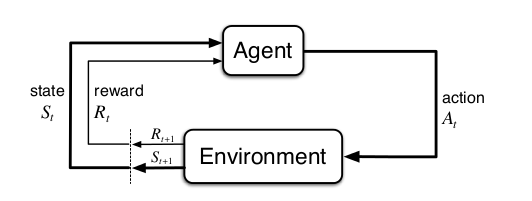
\includegraphics[scale=0.5]{assets/agent_environment_interface.png}
    \caption[]{Agent-Environment Interface}
    \label{fig:agent_environment_interface}
\end{figure}

The decision maker in this interface is called the \textbf{Agent}, and the agent interacts with the \textbf{Environment} continuously.
A problem implements the interface could be represented as a \textbf{Markov Decision Process (MDP)}, which is tuple of four elements where:
\begin{itemize}
    \item $\mathcal{S}$, a set of states that forms the \textit{state space}
    \item $\mathcal{A}$, a set of actions that forms the \textit{action space}
    \item $P(s, a, s') = Pr[ S_{t+1} = s' \mid  S_t = s, A_t = a]$, the transition probability function
    \item $R(s, a, s')$ the reward function
\end{itemize}
At each time step $t$, the agent starts at state $S_t \in \mathcal{S}$, picks an action $A_t \in \mathcal{A}$
transitions to state $S_{t+1} \in \mathcal{S}$ based on the probability function$P(S_{t+1} \mid S_t, A_t)$,
and receives a reward $R(S_t, A_t, S_{t+1})$.

The agent interacts with enviornment and generates a sequence of actions, states, and rewards:
$S_{0}, A_{0}, R_{1}, S_{1}, A_{1}, R_{2}, \dots$
We call this sequence a \textbf{trajectory}.
In the finite case, this interaction terminates until a terminal state is reached at time $t = T$, and this sequence is called an \textbf{episode}.
In the infinite case, the interaction continues indefinitely.
The goal of the agent in the problem is either to maximize the accumulative reward in the finite setting,
or to maximize the average reward in the infinite case.

\note{also describes policy $\pi$}

\note{address this is the most common formulation and how different libraries implement the interface}

\subsection{Shortcomings of the Agent-Environment Interface for General Game Playing}
% \note{I'm not sure if I should address these separatly.}
\subsubsection{Multi-Agent Games}
\note{address OpenSpiel's design multiple agents}
\subsubsection{Partial Observability}
\note{address POMDP}
\subsubsection{Environment Stochasticity}
\note{address OpenSpiel's design of random node}
\subsubsection{Episodic vs Continuous}
\note{barely seen in the literature, need more literature review}
\subsubsection{Self-Observability}
% \note{agent needs to be able to observe itself}
\subsubsection{Environment Output Structure}
% The agent-environment interface specifies two return types from the environment, namely the \textbf{observation} and the \textbf{reward}.
% All environment implementations used in the RL field follow 

\subsection{Our Approach}
\note{(5 pages)}

% The most significant difference of our approach is the separation of data and process.
% In the Agent-Environment Interface, both the agent and the environment are assumed to be stateful, which means they could store and process arbitrary data.

\subsubsection{Generalized Interaction Interface}
We propose the \textbf{Generalized Interaction Interface (GII)}.
We define the \textbf{tape} $E$ as the data storage of the interface, and a \textbf{law} $L$ as a pure function that operates on the tape.
An instance of such interface could consists of exactly one tape and multiple laws, and we define such an instance a \textbf{universe}.
A universe \textbf{ticks} by applying the laws on the tape.
\note{elaborate formally}

We implement a simplified version of this interface in \textbf{MooZi}.

% \note{elaborate on the interface}

\subsubsection{Advantages}
\note{pure functions are efficient}

\section{Method}
\note{(20 - 25 pages)}
\subsection{Design Philosophy}

\subsubsection{Use of Generalized Interaction Interface}
One of the goals of the project is to demostrate the use of Generalized Interaction Interface (GII).
All modules in the project will be implemented to align with the interface.
Third-party libraries that include game environments are wrapped with special wrappers that converts the outputs into the GII format.

\subsubsection{Use of Pure Functions}
One of the most notable difference of MooZi implementation is the use of pure functions.
In GII, \textbf{laws} are pure functions that read from and write to the \textbf{tape}.
Agents implemented in Agent-Environment Interface usually do not separate the storage of data and the handling of data.
In MooZi, we separate the storage of data and the handling of data whenever possible, especially for the parts with heavy compuations.
For example, we use \textbf{JAX} and \textbf{Haiku} to implement neural network related modules.
These libraries separate the \textbf{specification} and the \textbf{state} of a neural network.
The \textbf{specification} of a neural network is a pure function that is internally represented by a fixed computation graph.
The \textbf{parameters} of a neural network includes all variables that could be used with the specification to perform a forward pass.
\note{add one or two more examples of using pure functions, also mention how tape in the MooZi is different from the tape in GII}

\subsubsection{Being User Friendly}

\subsubsection{Training Efficiency}
One common problem with current open-sourced MuZero projects is their training efficiency.
Even for simple environments, these projects could take hours to train.
\note{
    Data needed; I've seen multiple issues on GitHub complaining about the training speed.
    I once assigned the task of "actually running the project and gather run time data" to Jiuqi but no follow up yet.
}

There are a few major bottlenecks of training efficiency in this type of project.
The first one is system parallelization.
\note{include data from previous presentation to make the point}

The second one is the environment transition speed.
\note{boardgames are fine, Atari games are slow, but in either cases we can't control}
% Board games, especially those are implemented in \textbf{OpenSpiel}, are faster.

The third one is neural network inferences used in training.
\note{MCTS inference batching is slow due to IO overhead, include data here from previous presentation to make the point}

% According to our deGeneralized Interaction Interface
\subsection{Structure Overview}

\begin{figure}[h]
    \centering
    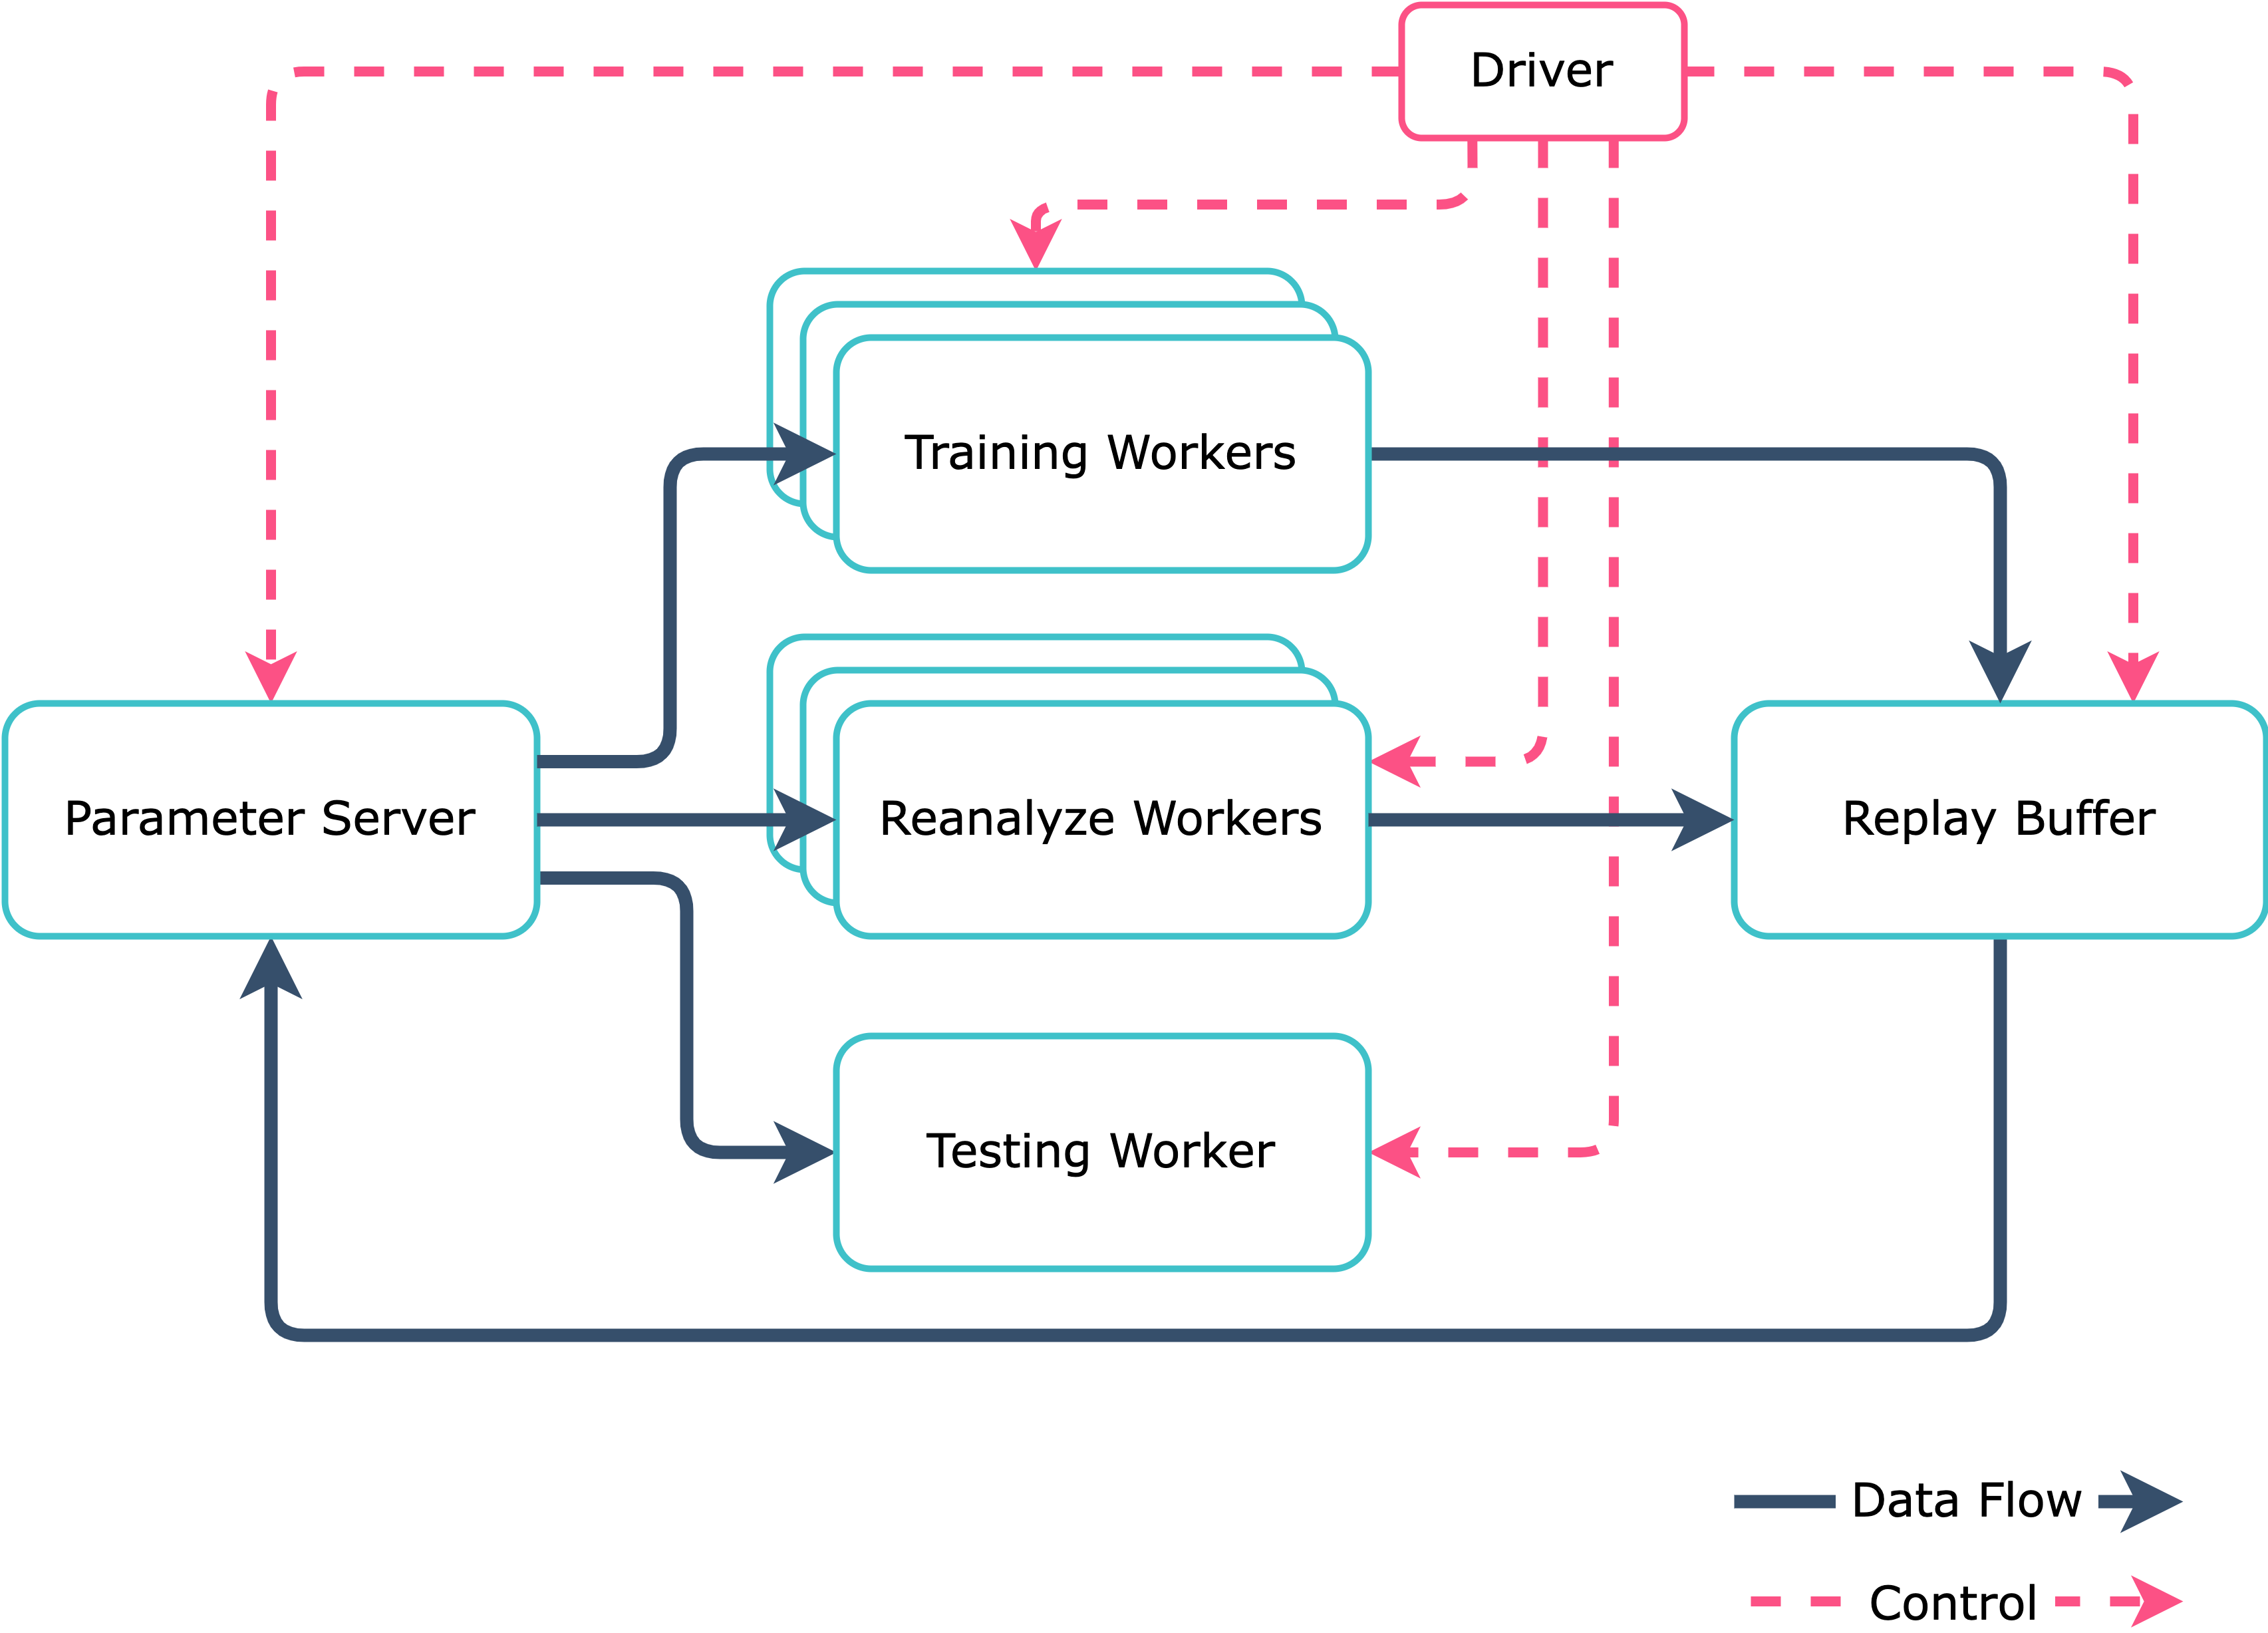
\includegraphics[width=\textwidth]{assets/moozi_architecture.png}
    \caption[]{MooZi Architecture}
    \label{fig:moozi_architecture}
\end{figure}

\subsubsection{Driver}
% MooZi adopts the \textbf{centralized control} design paradigm.
In a distributed system with centralized control, a single process is responsible for operating all other processes.
This central process is called the \textbf{driver}.
Other processes are either \textbf{tasks} or \textbf{actors}.
\textbf{Tasks} are stateless functions that takes inputs and return outputs.
\textbf{Actors} are statefull objects that group several methods that take inputs and return outputs.
In RL literature, \textbf{actor} is also a commonly used term to describe the process that stores a policy and interacts with an environment.
Even though MooZi does not adopt the concept of a RL actor, we will use the term \textbf{ray task} and \textbf{ray actor} to avoid confusion.
In contrast to distributed systems with distributed control, ray tasks and ray actors are reactive and do not have busy loops.
The driver decides when a ray task or ray actor is activated and what data should be used as inputs and where the outputs should go.
In other words, the driver process orchestrates the data and control flow of the entire system, and ray tasks and ray actors merely response to instructions.

\subsubsection{Environment Wrapper}

\subsubsection{Rollout Workers}
A \textbf{rollout worker} is a ray actor that:
\begin{itemize}
    \item stores a collection of universes, including tapes and laws in the universes
    \item stores a copy of the neural network specification
    \item stores a copy of the neural network parameters
    \item optionally stores batching layers that enable efficient computation
\end{itemize}

A rollout worker does not inherently serve a specific purpose in the system and its behavior is mostly determined by the list of laws created with the universes.

There are three main patterns of rollout workers used in MooZi:
\textbf{interaction training rollout worker},
\textbf{interaction testing rollout worker},
and \textbf{reanalyze rollout worker}.

\subsubsection{Replay Buffer}
The replay buffer:
\begin{itemize}
    \item stores trajectories generated by the rollout workers
    \item processes the trajectories into training targets
    \item stores processed training targets
    \item computes and updates priorities of training targets
    \item responsible for sampling and fetching batches of training targets
\end{itemize}

\subsubsection{Parameter Optimizer}
The parameter optimizer:
\begin{itemize}
    \item stores a copy of the neural network specification
    \item stores the latest copy of neural network parameters
    \item stores the loss function
    \item stores the training state
    \item computes forward and backward passes and updates the parameters
\end{itemize}

\subsubsection{Distributed Training}

\begin{python}
for epoch in range(num_epochs):
    for w in workers_env + workers_test + workers_reanalyze:
        w.set_params_and_state(param_opt.get_params_and_state())

    while traj_futures:
        traj, traj_futures = ray.wait(traj_futures)
        traj = traj[0]
        replay_buffer.add_trajs(traj)

    if epoch >= epoch_train_start:
        train_batch = replay_buffer.get_train_targets_batch(
            big_batch_size
        )
        param_opt.update(train_batch, batch_size)

    env_trajs = [w.run(num_ticks_per_epoch) for w in workers_env]
    reanalyze_trajs = [w.run() for w in workers_reanalyze]
    traj_futures = env_trajs + reanalyze_trajs

    if epoch % test_interval == 0:
        test_result = workers_test[0].run(120)

    for w in workers_reanalyze:
        reanalyze_input = replay_buffer.get_train_targets_batch(
            num_trajs_per_reanalyze_universe
            * num_universes_per_reanalyze_worker
        )
        w.set_inputs(reanalyze_input)
        
\end{python}

\note{explain driver pseudo-code}

\subsubsection{Monte-Carlo Tree Search}
%     - asynchronous
%     - batching layer

\subsubsection{Logging and Visualization}


\section{Experiments}
\note{(20 pages)}

\section{Conclusion}
\note{(3 pages)}
\subsection{Future Work}
\note{(1 page)}

\end{document}

\subsection*{Artificial Intelligence}

% Artificial Intelligence (AI) is a branch of computer science that emphasizes the use of computer algorithms to solve problems likes humans.
To define the goals and methods of Artificial Intelligence (AI), we first need to define what is \textit{intelligence}.
Though there is no consensus on the exact definition of intelligence, here we adopt the definition by John McCarthy:
\begin{quote}
    Intelligence is the computational part of the ability to achieve goals in the world.
\end{quote}
The goal of AI is to develop computer algorithms that can solve problems and achieve goals in complex environments.
A diverse range of methods are designed as AI algorithms since the term has been coined.
\note{A simple list of AI algorithms, such as A*, symbolic}


\subsection*{Game Artificial Intelligence}
Perfect vs in-Perfect information
\subsection*{Planning}
lookahead search: A*, DFS, BFS

\subsection*{Distributed System for AI}
IMPALA, SEED
